\section{Theorie}
\subsection{Theorie des Lichts}
Ein Laser emittiert hoch intensives monochromatisches Licht, also Licht einer einzigen Wellenlänge beziehungsweise Farbe. Außerdem muss das Licht kohärent sein, also den Kontrast der Interferenzmuster maximieren. In der Realität ist das Licht nicht perfekt monochromatisch, da im Lasergehäuse die Neonatome nicht still stehen, sondern eine eigene Geschwindigkeit haben und somit der Doppler-Effekt bezüglich des emittierten Lichts eintritt. Somit ist auch die perfekte Kohärenz nicht möglich.

\noindent Licht wird im Teilchenbild durch Emission von Photonen beim Übergang eines Elektrons von einem Niveau eines Atoms in ein energetisch günstigeres beschrieben. Es existieren zwei Arten der Emission. Die stimulierte und spontane Emission. Die spontane Emission entsteht durch Fluktuationen in der Ladungsverteilung der Atome. Die stimulierte Emission ist die für den Laser relevante, da dabei im Gegensatz zum statistischen Ereignis der spontanen Emission, die Abstrahlung von Photonen kontrolliert werden kann. Durch das Auftreffen eines Photons wird der Übergang eines Atoms in einen Zustand geringerer Energie, unter der Voraussetzung, dass das Photon die Energie der Energiedifferenz zwischen aktuellem Zustand und dem energetisch günstigerem hat, ermöglicht. Es wird zusätzlich zu dem einfallenden Photon ein weiteres Photon durch den Übergang emittiert. 

\noindent Darüber hinaus gibt es noch die Absorption. Hierbei wird ein auf das Atom treffende Photon, welches die Energie des Überganges hat, absorbiert, indem ein Elektron in ein der Photonenenergie entsprechend höher liegendes elektronisches Niveau wechselt.

\noindent Ein zwar nicht für die Funktion eines Lasers ausreichendes, aber grundlegendes System ist das Zwei-Niveau-System. Dabei wird die Besetzungsdichte \(n_2\) des angeregten Zustandes durch die Absorption erhöht und durch die spontane und stimulierte Emission verringert. Um hochintensive Licht zu erzeugen, muss bei einem Laser die stimulierte Emission der spontanen überwiegen, sodass das \(n_2>n_1\) ist, wobei \(n_1\) die Besetzungsdichte im Grundzustand bedeutet.

\subsection{Theorie des Lasers}
Ein Laser besteht im wesentlichen aus drei Komponenten. Eine ist das aktive Lasermedium. Dabei handelt es sich um ein Gas, einen Festkörper oder eine Flüssigkeit. Bei dem Laser dieses Versuchs wird ein Gas verwendet. Die notwendige Bedingung an ein Lasermedium stellt die Fähigkeit zur Besetzungsinversion dar, also \(n_2>n_1\). Als Lasermedium dient hier Neon.

\noindent Eine weitere Komponente ist die Pumpquelle. Durch das so genannte Pumpen, wird dem Lasermedium Energie zugeführt und somit Zustände höherer Energie häufiger besetzt, als diejenigen niedrieger. Es wird also eine Besetzungsinversion erzeugt. Helium ist hierbei das Pumpgas. Mit einer Spannungsquelle wird das Helium mittels elektrischer Entladung in metastabile Zustände angeregt. Die Energie wird dann vom Helium an das Neon durch Stöße zweiter Art übergeben. Diese sind Stöße zweier Atome, von denen eines im Angeregten und das andere im Grundzustand ist. Bei einem Stoß zweiter Art besteht dann eine Wahrscheinlichkeit, das angeregte Atom in den Grundzustand und das im Grundzustand verweilende in den angeregten Zustand zu bringen. 

\noindent Die dritte Komponente ist der Resonator. Er besteht aus einem möglichst vollständig reflektierenden und einem teildurchlässigen Spiegel sowie einem Laserrohr, in dem sich das Lasermedium befindet und das an den Enden in Brewsterfenstern mündet. Die Spiegel stehen in einem Abstand \(L\)  voneinander entfernt auf der optischen Achse und haben die Krümmungsradien \(r_1\) und \(r_2\). Dadurch entsteht eine optische Rückkopplung, bei der das Licht mehrmals das Lasermedium durchläuft und ein selbsterregender Oszillator entsteht. 

\begin{figure}
	\centering
	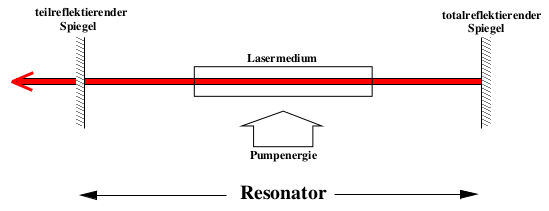
\includegraphics[width=0.75\textwidth]{img/resonator}
	\caption{Laser-Resonator \cite{V61}}
	\label{fig:resonator}
\end{figure}

\noindent Die Abbildung \ref{fig:resonator} zeigt einen groben Aufbau eines Resonators.

\noindent Durch den Resonator legt der Laserstrahl einen möglichst langen Weg im Lasermedium zurück und wird somit verstärkt. Optimal ist für einen Laser ein konfokaler Resonator, da die Brennpunkte der Spiegel zusammenfallen und somit die Verluste minimiert werden.

\noindent Eine Stabilitätsbedingung für den Resonator ist gegeben durch:

\begin{equation}
0\le g_1\cdot g_2<1
\end{equation}

\noindent Dabei sind die \(g_i\) durch \(g_i=1-\frac{L}{r_i}\) gegeben.

\noindent Es existiert eine Mehrzahl von Frequenzen, die die Resonanzbedingung erfüllen. Diese sind über 

\begin{equation}
\label{eq:q}
f=\frac{nc}{2L}
\end{equation}

\noindent gegeben. Es gibt sowohl transversale als auch longitudinale Moden. Erste entstehen durch Unebenheiten der Spiegel oder Verkippungen und sind im Wesentlichen eine Intensitätsverteilung elektromagnetischer Strahlung, die senkrecht zur Ausbreitungsrichtung dieser gemessen wird. Die Moden werden als \(\text{TEM}_{lpq}\) (transverse electromagnetic mode) bezeichnet, dabei sind \(l\) und \(p\) die Knoten in x- und y-Richtung und heißen transversale Modenzahl. Das \(q\) steht für die Anzahl der longitudinalen Moden, welche dann für das \(n\) in Formel \ref{eq:q} eingesetzt werden. Die Verluste steigen mit der Modenzahl, sodass nur wenige Moden isoliert werden können. Die Mode mit höchster Symmetrie und mit den wenigsten Verlusten ist die \(\text{TEM}_{00}\) Grundmode, die über eine Gaußverteilung gegeben ist:

\begin{equation}
\label{eq:gauß}
I(d)=I_0\cdot e^{-2\left(\frac{d-d_0}{w}\right)^2}\quad.
\end{equation}